\documentclass[sigconf, review=true]{acmart}
\usepackage[english]{babel}
\usepackage{graphicx}
\graphicspath{ {./images/} }
\author{Jeroen-Niclas Trzaska}
\title{DB proseminar - Isolation Levels}
\acmDOI{}
\acmISBN{}
\affiliation{%
   \institution{TU Dresden}
   \city{Dresden}
   \state{Saxony}
   \country{Germany}}
\email{jeroen@trzaska.xyz}

\citestyle{acmauthoryear}
\begin{document}

\begin{abstract}
    This paper is going to look at the strengthened ANSI definition propositions by \cite{Adya_Liskov_O_Neil_2000} as well as the corresponding isolation levels,
    comparing them in terms of strength. We will also take a quick look at non lock based implementations
    and the problems the ANSI standard has in regards to such implementations as shown in \cite{Berenson_Bernstein_Gray_Melton_O_Neil_O_Neil_1995}.
\end{abstract}
\maketitle

\section{Motivation}
The motivation behind these analyses of the ANSI standard is to better define and examine the
behavior of different database implementation approaches when presented with multi-item dependencies.
This is important as the ANSI standard was created when locking implementations where the norm and thus multi version systems were not
taken into account creating it leading to a behavior not in line with ANSI.
These issues include but are not limited to dependency constrains between two items.

For example assume that Alice has two accounts at a bank. She has 20€ on each of them. Now she withdraws 30€ from account A and another 20€ form account B.
Looking at each of the transactions we can see that the constraint $A+B \geq 0$ is met.
But when executed simultaneously the resulting sum can still be negative. To do so
she asked Bob to help her.
\begin{example}
    Alice reads 20€ to be in both accounts and Bob does the same. Alice then withdraws 30€ from account A and writes -10€ into it and commits, the constrain is still met.
    Bob then withdraws 20€ from account and, as his transaction read both accounts to have 20€, he writes 0€  to B. This now violates the constrain $A+B \geq 0$.
\end{example}
\section{Phenomena Definitions}
We are now going to introduce the strengthened ANSI phenomena definitions as described in \cite{Adya_Liskov_O_Neil_2000}  which
are based on the broad interpretation of the ANSI standard. These definitions are inherently stronger then their ANSI counter part,
as they rule out other Phenomena not defined in the following paragraph. This is due to the fact that the ANSI standard
was created with locking implementations in mind. Leading to definitions that would allow phenomena to appear in the database history when using non lock based systems
while lock based systems using the same interpretation would not.

\subsection{P0 - Dirty write}
An example for the above mentioned problem with ANSI strength is that while a locking implementation of read uncommitted
prevents the following phenomenon, a non locking system would not do so.
So lets start by defining the first phenomena, which describes two consecutive writes by two different
transactions leading to an unclear value for X when the first transaction aborts.

\begin{figure}[h]
    
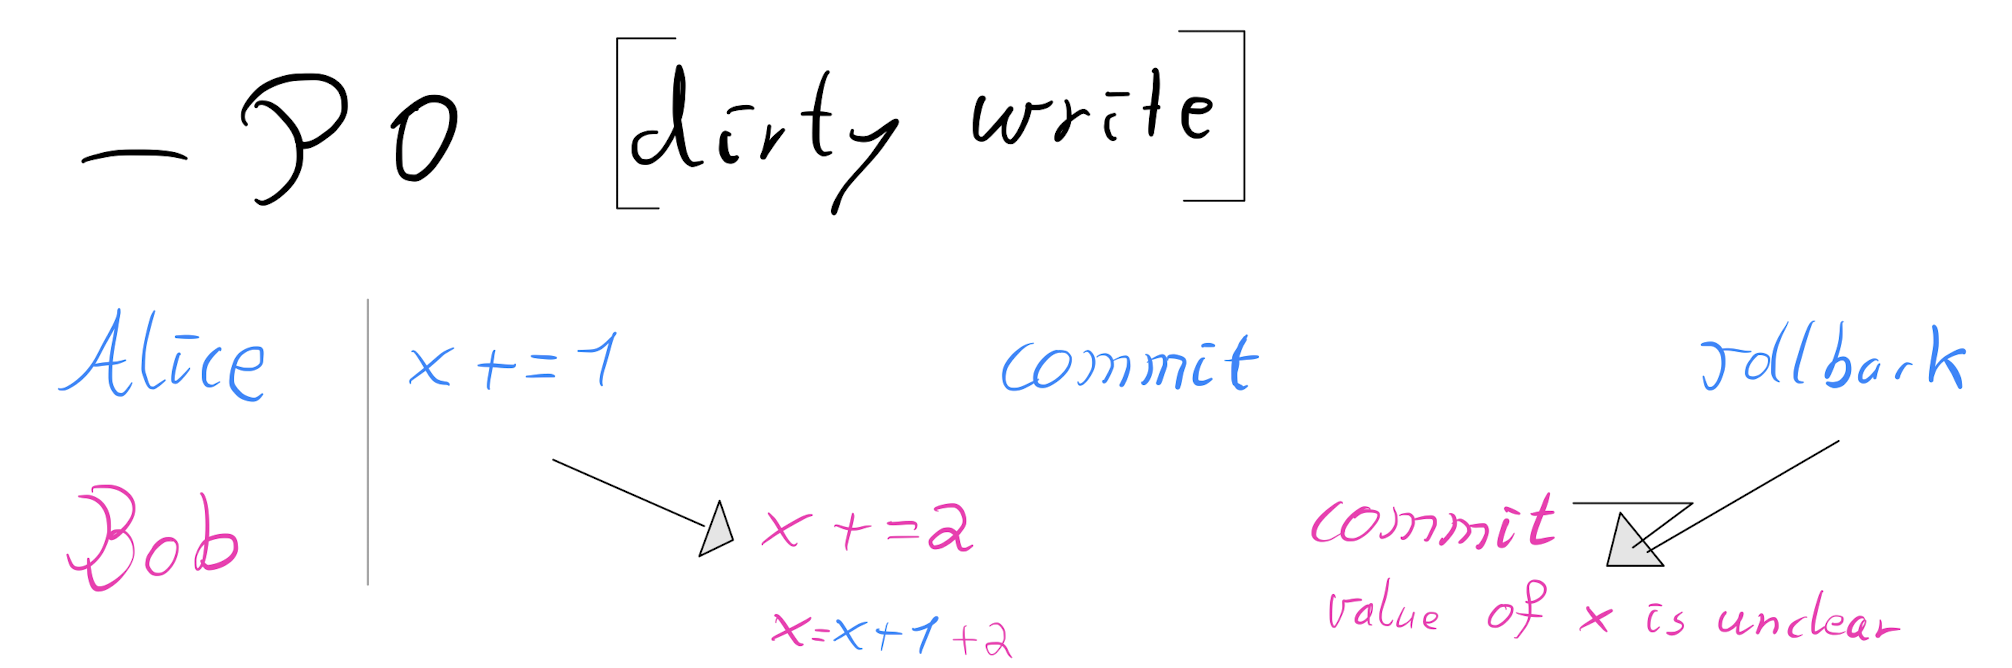
\includegraphics[width=8.5cm]{P0}

\end{figure}

\begin{example}
    Alice deposits 10€ into a bank account X.
    Bob than deposits a further 20€ into the same account.
    To do so he reads the value of X and then adds 20€ and writes it back to the account X.
    Alice than performs a rollback on her transaction.
    Thus the amount of money in account X is unclear.
\end{example}

\subsection{P1 - Dirty read}
For the second phenomenon we are going to look at reading inconsistent data.
This can be a problem when retrieving information while another transaction
that writes data is being executed. An issue that can arrive due to this phenomena is
that the given transaction reading the inconsistent data might continue to work with this
incorrect data and writing wrong data back to the database, corrupting it in the process.


\begin{figure}[h]
    
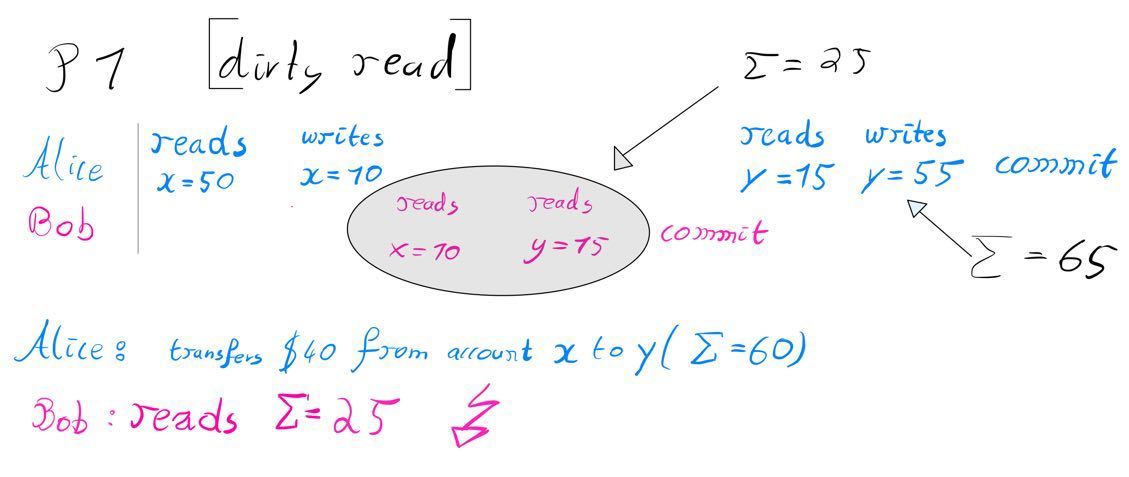
\includegraphics[width=8.5cm]{P1}
    
\end{figure}

\begin{example}
    Alice transfers 40€ form account x to account y.
    To do so she reads the value of x subtracts the 40€ writing 10€ to value x.
    Afterwards, Bob reads the value of x (10€) and y (15€) resulting in a sum of 25€
    Alice then reads the value of y (15€) and then adds the 40€ to it resulting in a 55€ sum for y
    and a total of 65€.
\end{example}

\subsection{P2 - Fuzzy read}
The next phenomenon is similar to P1 as it has to do with read inconsistencies, too.
Though this time performing the two reads of the reading transaction without interruption would lead
to the correct data, so the read is non repeatable. This is an issue as the transaction does not know that
it was interrupted and assumes that the data in the database has not changed. Thus it operates under a false pretense
and might corrupt the database when writing data back to it.

\begin{figure}[h]
    
    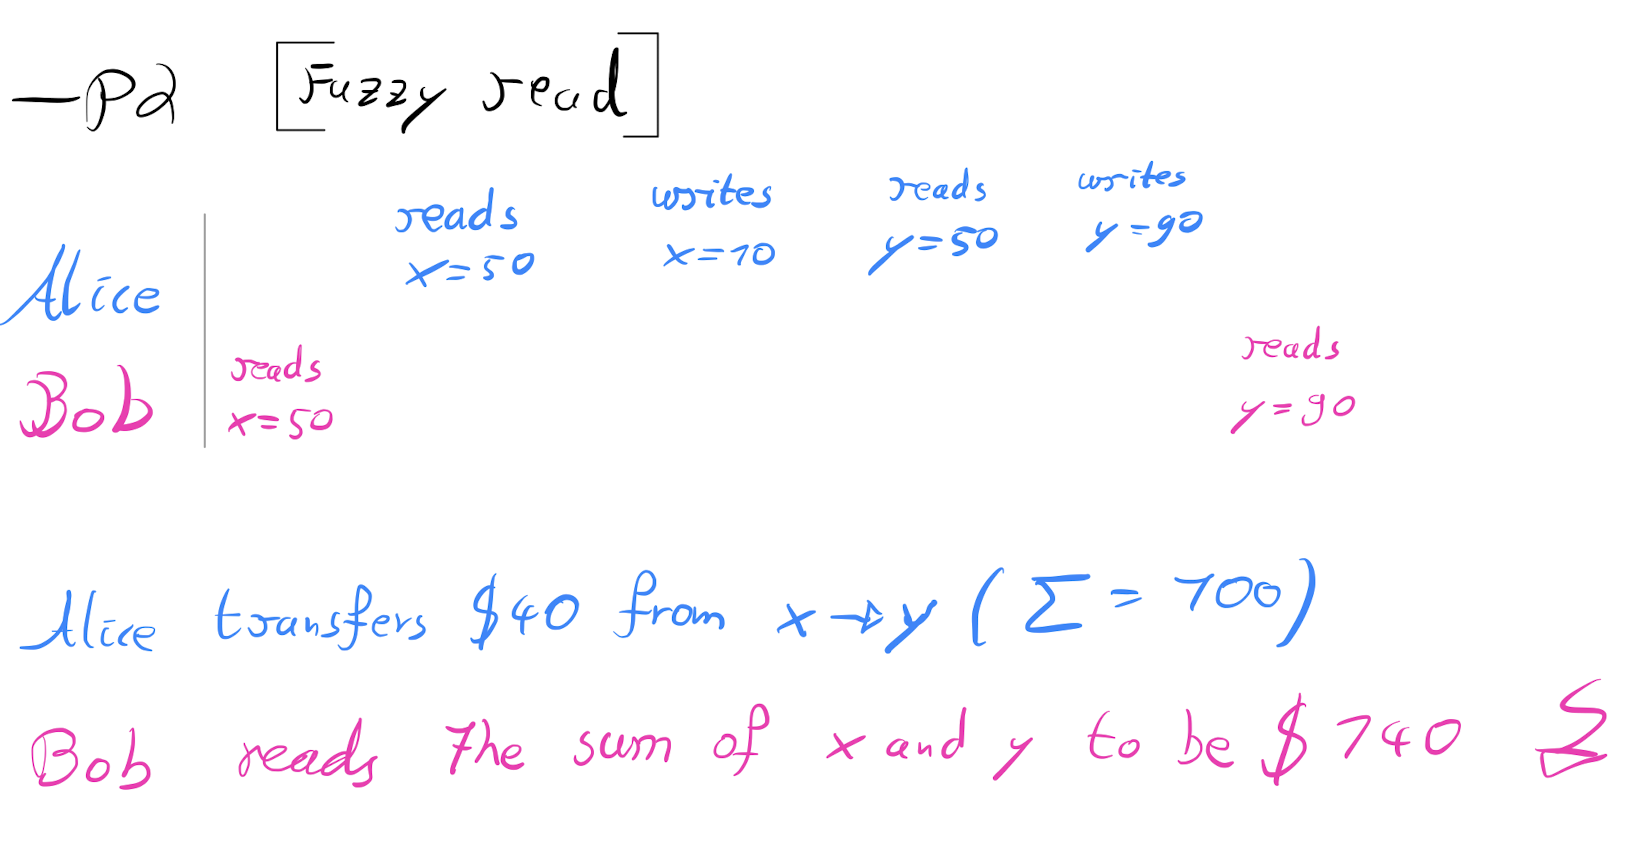
\includegraphics[width=8.5cm]{P2}
    
\end{figure}

\begin{example}
    Bob starts to read the sum by reading x and gets interrupted by Alice who then transfers 40€ from x to y. 
    After this is completed Bob reads the value of y.
    Thus the sum is 100€ for Alice and 140€ for Bob.
    In contrast to P1 a second read of x by Bob would have returned the correct sum.
\end{example}
\subsection{P3 - Phantom}
Once again when looking at the ANSI specification one can see that it only disallows inserts on the serializable
isolation level while the following definition of P3 prohibits deletions, inserts, and updates, making it stronger than A3.
This phenomenon is only applicable to transactions using predicates and applies to deletions, insets, and updates.


\begin{figure}[h]
    
    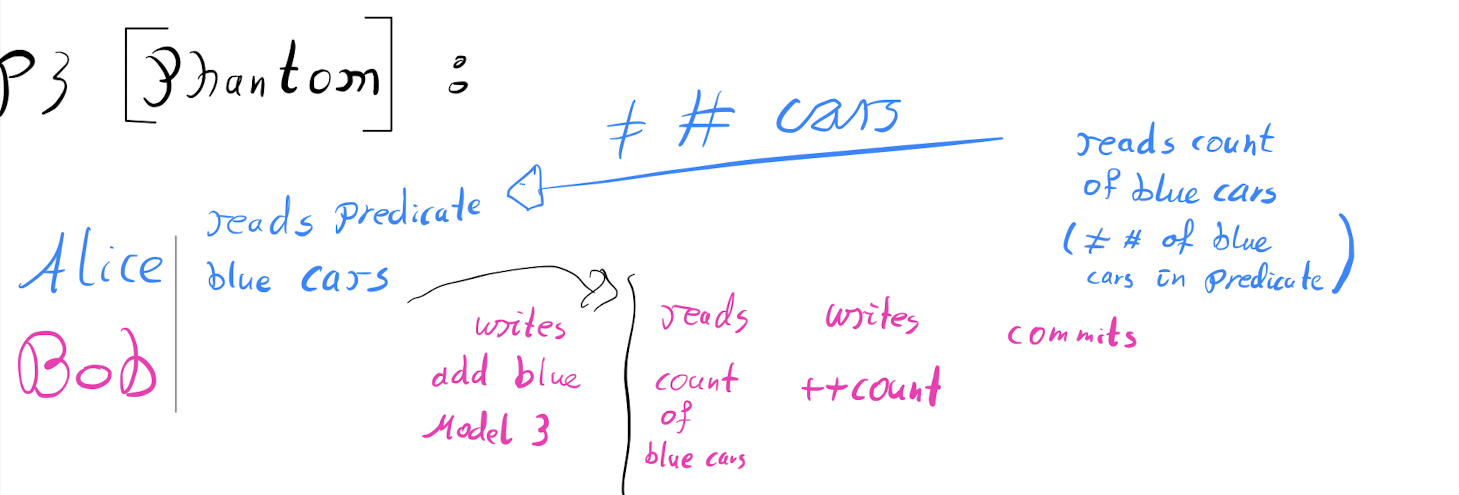
\includegraphics[width=8.5cm]{P3}
    
\end{figure}

\begin{example}
    Alice reads the predicate blue cars. Bob then adds a new blue car to the database and increases
    the count of blue cars. Alice then reads the count of blue cars. This leads to a phantom item
    (Alice can’t see Bob's car but knows of its existence due to the increased count).
\end{example}
Not prohibiting this phenomenon can cause inconsistent predicate reads and in the worst case phantom entries in the
database as the reading transaction could, after reading a phantom object, either assume that it does not exist or treat it like an actual
object, both situations would lead to undefined behavior of the transaction.

\section{ANSI isolation levels}
We define the isolation levels by the phenomena prohibited by it and we define
Degree 0 isolation to be the isolation level that does not prohibit any abnormal
behavior. Furthermore, we define short duration locks as locks that are held
while a transaction reads or writes an item, in contrast to long-duration locks which are
held until a transaction commits or aborts.
These definition can then be used to classify different database system implementations in
regards to their serializability.

\subsection{Read uncommitted}
We define read uncommitted to be the isolation level that prohibits the phenomenon
P0, dirty write. This can be accomplished by placing \emph{long-duration write locks} when modifying a data item.
This only allows one transaction at a time to write to a given value and requires all others to wait for a commit or abort.

\subsection{Read committed}
Read committed is defined as the isolation level where P1, dirty read, is prohibited.
To accomplish this the use of \emph{short duration read locks}, as well as long write locks, is
necessary. Thus disallowing a write on data that was just read by another transaction as
well as disallowing overwriting of an item already written by another, not finished, transaction.

\subsection{Repeatable read}
For repeatable read, the phenomenon P2, fuzzy read, has to be prohibited.
This requires \emph{long duration write locks} as well as \emph{long duration read locks} on
items and short ones for predicates.\\
The difference to read committed is that read committed only guarantees that
the data read was committed at the time of reading (no dirty reads), whereas
repeatable read also guarantees that the data will not change before the
transaction finishes either with a commit or abort.


\subsection{Serializable}
For serializability P3 needs to be prohibited, which can be done by placing \emph{long locks
on reads and writes}. This isolation level is stronger then it's ANSI counter part due to the
prohibition of predicate updates and deletions as defined in P3, making it the only isolation level
outside of the original ANSI isolation level specifications.

\section{Cursor stability}
For the cursor stability, it is useful to define a fourth phenomenon P4 (lost update), as this isolation level
was designed to solve the problem of lost updates.
\subsection{ P4 - lost update}
This phenomenon describes the loss of an update by a transaction due to it immediately being overwritten
by a second transaction.

\begin{figure}[h]
    
    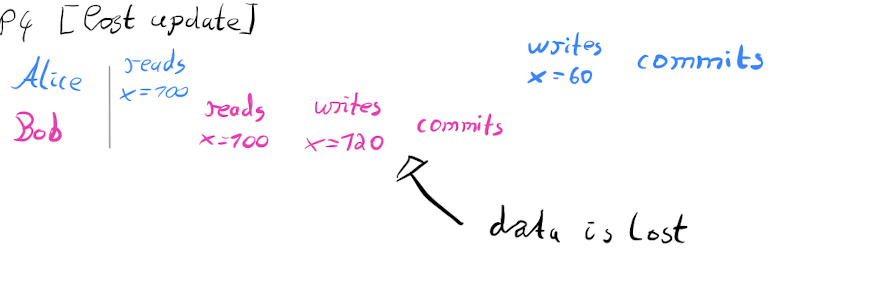
\includegraphics[width=8.5cm]{P4}
    
\end{figure}

\begin{example}
    Alice reads x to be 100€. Bob then reads the same, adds 20€ and writes 120€ to x and commits.
    Alice then subtracts 40€ from x and writes 60€ to x and commits, resulting in the loss of Bob's update.
\end{example}
\subsection{Implications}
    The phenomena define above can be prohibited when a read lock is placed on x (position of the cursor) when
    read and placing a long write lock on the items row when modified.
    The read lock is removed when the cursor moves (e.g. reading a new cell),
    while the write lock only gets removed after the transaction commits or aborts.
    As Cursor stability is stronger then read committed while being weaker then repeatable read, it
    is used instead of the weaker repeatable read by some database systems. This behavior is allowed by the ANSI standard
    as it defines a minimum set of guarantees.
\subsection{Strength}
When looking at our isolation levels defined in section 2, we can see that P4 is prohibited by repeatable read,
as long duration locks on read and write will also disallow the overwriting of an item by another transaction.
It is thus weaker than repeatable read as prohibiting P4 does not prohibit P3.
Looking at read committed, one can reason that one transaction A can read X, then be interrupted by transaction B which updates
item X and commits, and transaction A then continues to write to X.
Thus making Cursor stability stronger than the strengthened read committed.
\subsection{Multi cursor}
While the Cursor stability based system described above could also be extended with the use of multiple cursors, thus
parleying the effect of repeatable read isolation as long as each transaction does not access more items
then the system has cursors. But obviously this is not a general, or even practical solution to the phenomenon P2 and
although it might have real life use cases it wo not be discussed further in this paper.
\section{Snapshot Isolation}
All of the above-mentioned systems suggest lock-based implementations. In contrast we will also look at
snapshot isolation which uses multi-versioning.
In snapshot isolation, each transaction gets its own snapshot of committed data at the start.
Thus reads are never blocked, while writes are performed on the given snapshot as to not disturb
other transactions and allow reads of the updated data only by the same transaction (unless committed).
For the committing procedure, a second (commit) timestamp is assigned, said timestamp is larger than every
other assigned time stamp in the system. If another transaction A already modified data of the committing
transaction B it's commit fails, leading to an abort.
\subsection{P5B - Write skew}
To take a closer look at the difference to repeatable read it is useful to define a new phenomenon.

\begin{figure}[h]
    
    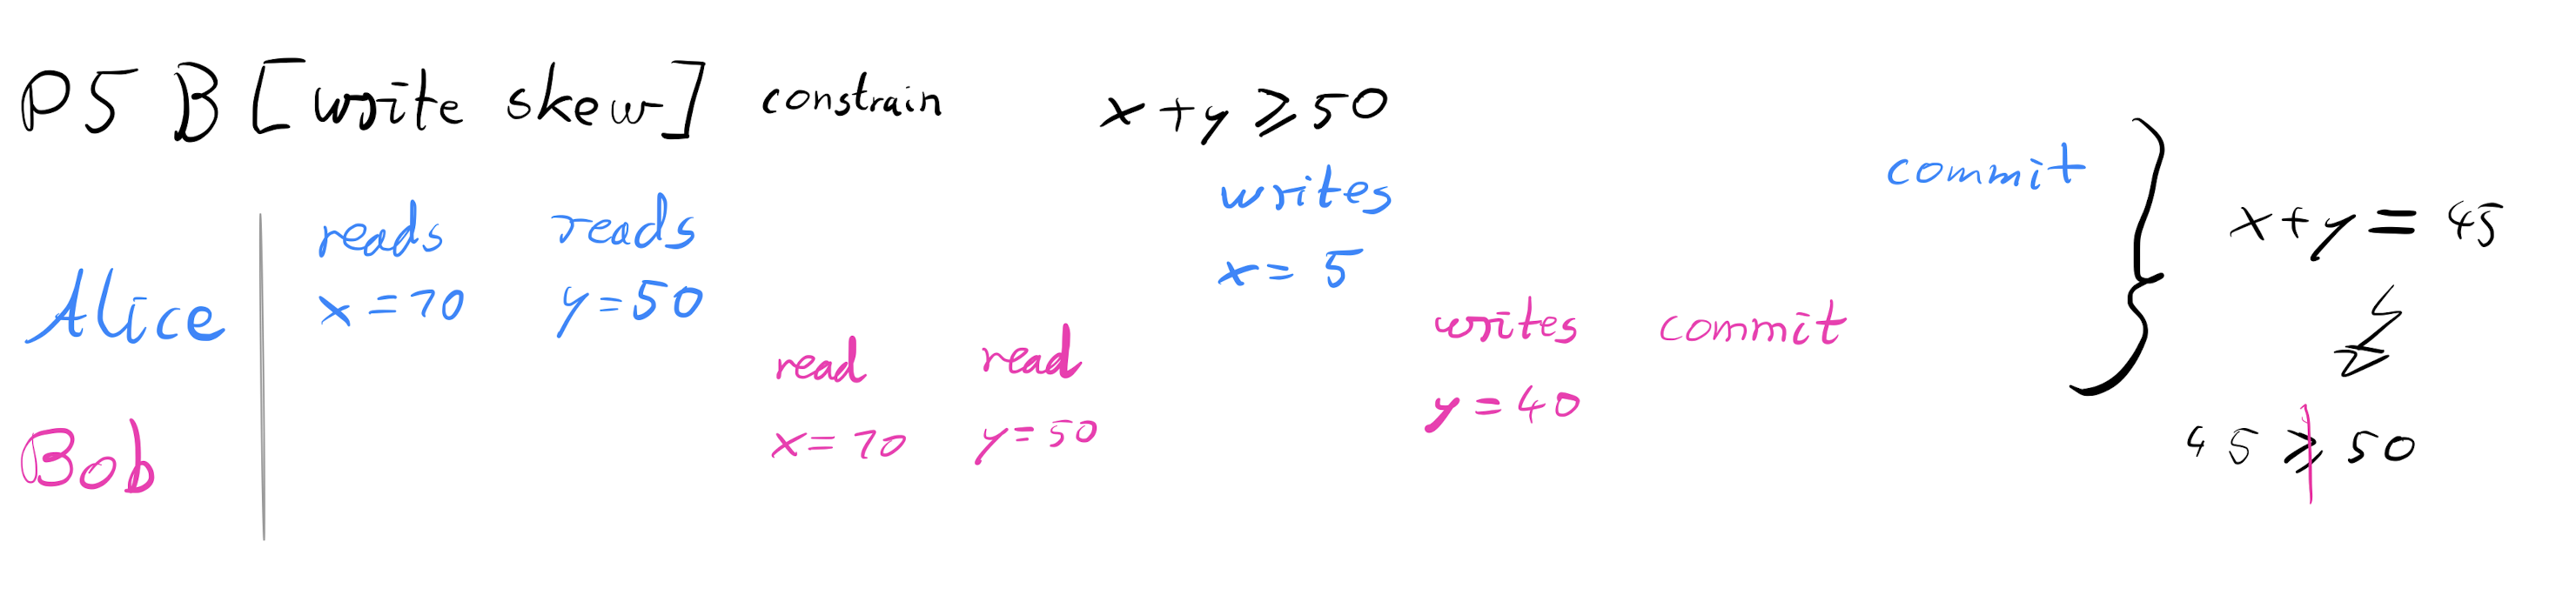
\includegraphics[width=8.5cm]{P5}
    
    \end{figure}
\begin{example}
    (first commit wins):
    Constraint: $ X+Y \geq  50$
    Alice reads x to be 10€ and y to be 50€. Bob then reads the same data, while getting his own snapshot
    to operate on (newer timestamp than Alice). Alice then sets x to be 5€,
    resulting in a sum of 55€. Bob then sets y to be 40€. Alice commits and Bob then tries to commit.
\end{example}
This would be prohibited by repeatable read but is allowed in snapshot isolation.
\subsection{Implications}
When looking at the phenomena defined above one can see that prohibiting it with a locked based system
would be the same as prohibiting P3 as a lost update can only be prohibited by placing long locks.
But when using a multi version system instead proscribing P5B is not equal to proscribing P3.

The example in subsection 5.1 is allowed by Snapshot isolation as it does not check for constrains and the transaction
does not modify the same item (x and y respectively). Repeatable read on the other hand would disallow such
behavior as it places long read and write locks on the items.
P5B is thus useful to differentiate between Snapshot isolation and repeatable read.
\subsection{Comparison with repeatable read}
As stated above repeatable read prohibits P5B while snapshot isolation prohibits some cases of
P3 and both prohibit P0, P1, and P2. Although the argument above is made with a locking implementation
it is general as the phenomena defined were strengthened to match the locking behavior.
\subsection{Strength}
Snapshot isolation is comparable in strength to repeatable read as both prohibit P0, P1, and P2.
To further investigate their difference we have to take a look at the original ANSI specification of serializable,
as it prohibits A3, which will be defined in the following section.
\subsection{A3 - Anomaly Phantom}
This is the strict interpretation of the Phantom anomaly. The difference to P3 is that the position of the
transactions commit is not indifferent for A3.
\begin{example}
    Alice reads the predicate blue cars. Bob then adds a new blue car to the database and increases
    the count of blue cars. Bob commits.  Alice then reads the count of blue cars. This leads to a phantom item
    (Alice can’t see Bob's car but knows of its existence due to the increased count).
\end{example}
Thus A3 only operates on committed data while P3 accounts for transactions to still be in progress,
making A3 a weaker phenomenon than P3.
\subsection{Comparison to ANSI}
When looking at the weak interpretation of the ANSI specification as in \cite{Adya_Liskov_O_Neil_2000}
one can see that Snapshot isolation prohibits all three anomalies A1, A2, and A3 making it ANOMALY SERIALIZABLE.
To show this we will now take a look at A3 as we have already shown above that Snapshot isolation prohibits P1 and P2.
As the definition of A3 states the importance of commit sequence it is easy to see that Snapshot isolation with a first commit wins
strategy precludes A3, as a already altered item will lead to an abort.
When looking at a first write wins the same is true as still only one modified value will
be written to the database and the other one will be discarded by an abort. It thus only changes
which transaction wins in comparison to first commit wins.
\subsection{Comparison to Serializable}
In comparison to the serializable isolation level defined in section 3.4 we can say that Snapshot isolation is
weaker as serializable precludes P5B as well as P3, which as shown in example 5.1 above does not hold true
for Snapshot isolation.
\section{Conclusion}
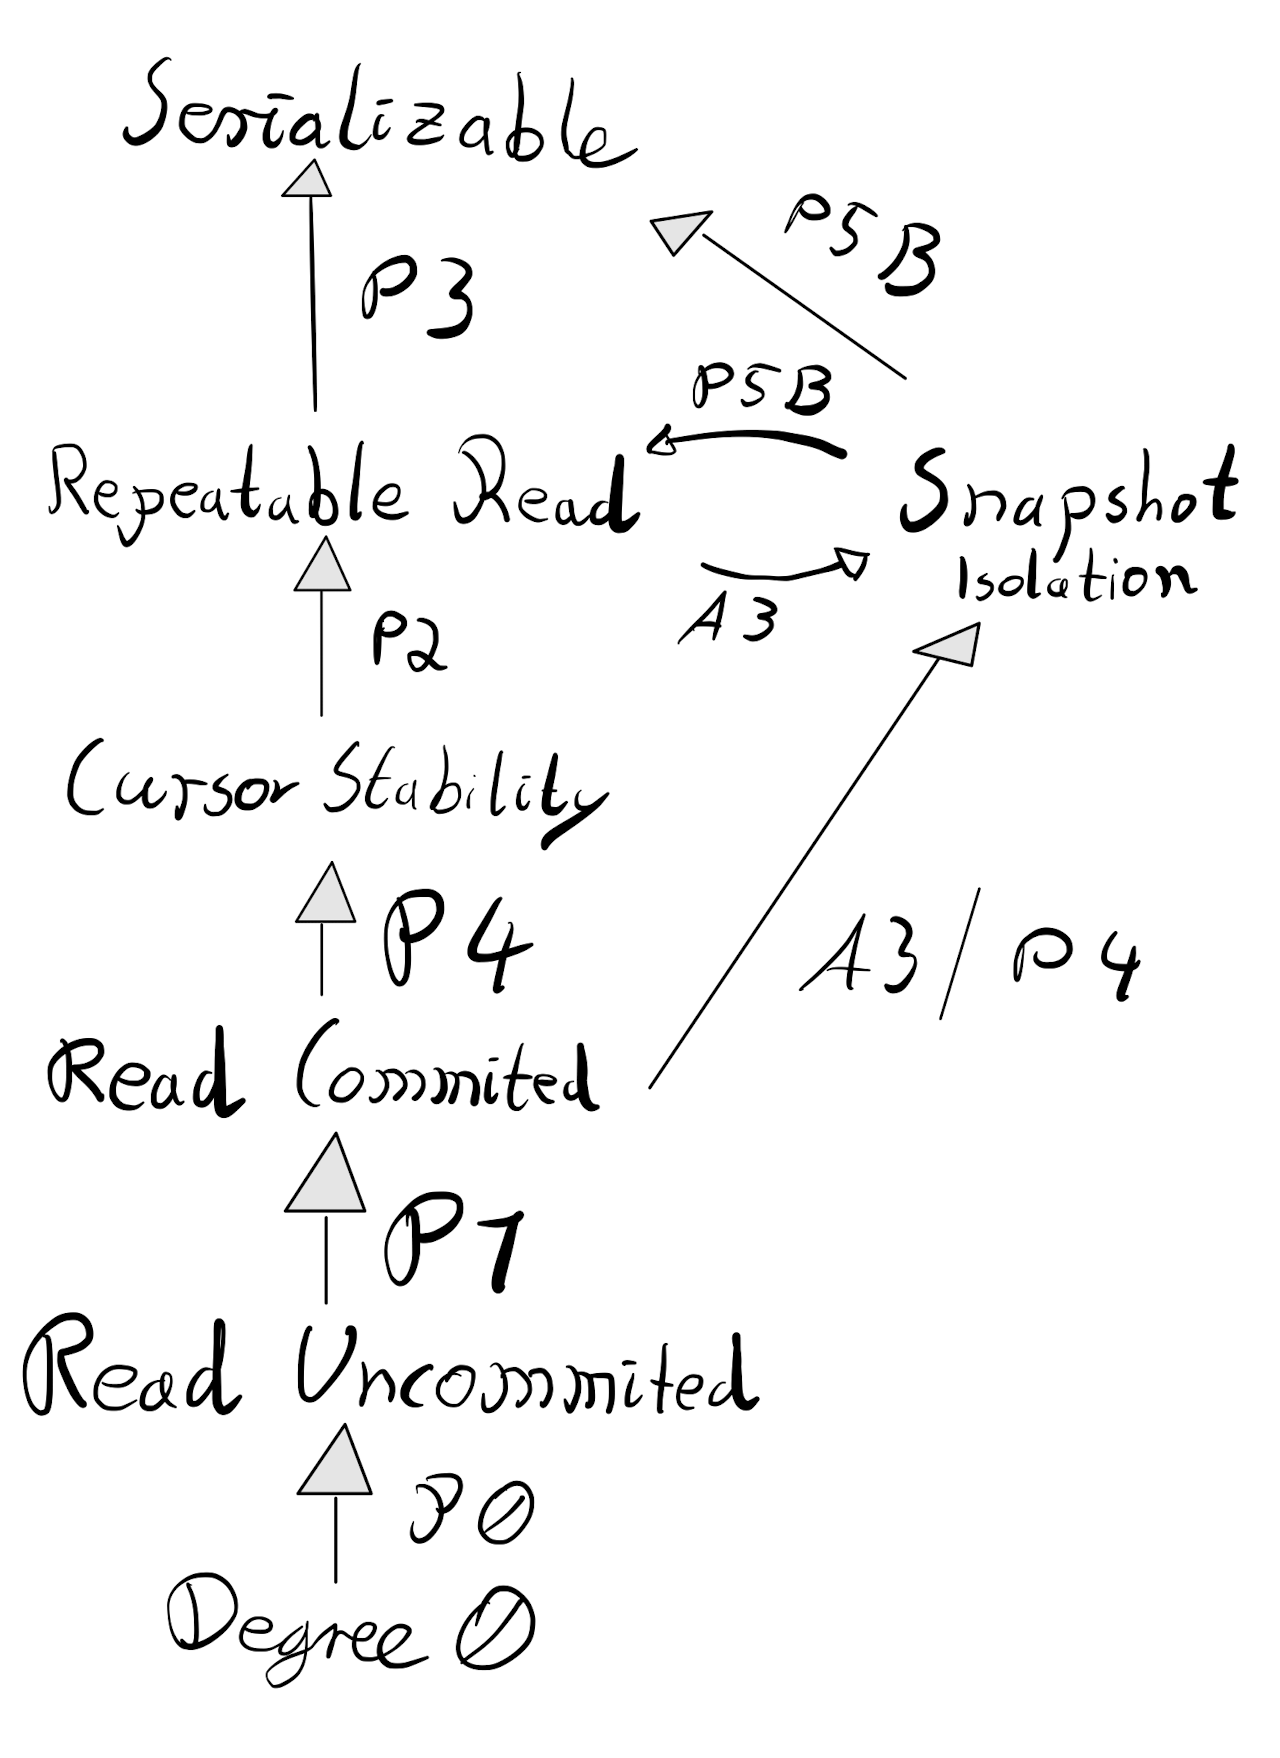
\includegraphics[width=8cm, height=8cm]{iso_lvl_dia.png}

In conclusion one can see that the ANSI specification is inherently flawed when talking
about multi-version histories and non locking database systems, as it failed to consider
these systems when defining the phenomena. As this will inevitably lead to different interpretations
and implementations it might be advisable to update the ANSI standard
according to the definitions given in \cite{Adya_Liskov_O_Neil_2000} and \cite{Berenson_Bernstein_Gray_Melton_O_Neil_O_Neil_1995}
to ensure the correct behavior of non locking implementations of ANSI SQL.
\bibliographystyle{plainnat}
\bibliography{refs}

\end{document}